%%%%%%%%%%%%%%%%%%%%%%%%%%%%%%%%%%%%%%%%%%%%%%%%%%%%%%%%%%%%%%%%%%%%%%%%%%%%%%%%%%%%%%%%%%%%%%%%%%%%%%%%%%%%%%%%%%%%%%%%%%%%%%%%%%%%%%%%%%%%%%%%%%%%%%
% 20141003 - Introduction to Operating Systems VO
%%%%%%%%%%%%%%%%%%%%%%%%%%%%%%%%%%%%%%%%%%%%%%%%%%%%%%%%%%%%%%%%%%%%%%%%%%%%%%%%%%%%%%%%%%%%%%%%%%%%%%%%%%%%%%%%%%%%%%%%%%%%%%%%%%%%%%%%%%%%%%%%%%%%%%

\tikzstyle{block} = [rectangle, draw, fill=blue!20, 
    text width=10em, text centered, rounded corners, minimum height=3em]
\tikzstyle{info} = [rectangle, draw, 
    text width=10em, text centered, rounded corners, minimum height=3em]

%fancyhdr
\lhead{IOS VO} 
\rhead{2014-10-03}

%%%%%%%%%%%%%%%%%%%%%%%%%%%%%%%%%%%%%%%%%%%%%%%%%%%%%%%%%%%%%%%%%%%%%%%%%%%%%%%%%%%%%%%%%%%%%%%%%%%%%%%%%%%%%%%%%%%%%%%%%%%%%%%%%%%%%%%%%%%%%%%%%%%%%%

\par{
    \noindent
    \underline{Example:}
    \par{
        \noindent
        \begin{tabular}{lll}
            \hline
            C Code                  &   Instructions                &    Additional information                             			\\
            \hline
            \hline
            \rowcolor{blue!25}                
            \texttt{while(x<1) \{}	&   \texttt{LDW 1, 28, -4}     	&   R1 := x                               							\\
            \rowcolor{blue!25}
            \texttt{{  }<body>}		&   \texttt{ADDI 2, 0, 1}       &   R2 := 1                                             			\\
            \rowcolor{blue!25}
            \texttt{\}}				&   \texttt{CMP 1, 1, 2}        &   R1 := R1 - R2                                    				\\
			\rowcolor{blue!25}
									&	\texttt{BGE 1, 0, 0}		&	\texttt{c} is set to zero, because at this point of time		\\
			\rowcolor{blue!25}
									&								&	we don't know where to jump to (in general).					\\
			\rowcolor{blue!25}
									&								&	A FixUp will later update this address.							\\
			\rowcolor{blue!25}
									&	\texttt{<body>}				&	The body of the function										\\
			\rowcolor{blue!25}
									&	\texttt{BR 0, 0, <top>}		&	\texttt{<top>} is the address offset to branch BEFORE 			\\
			\rowcolor{blue!25}
									&								&	the first generated instruction (\texttt{LDW 1, 28, -4}).		\\
            \hline
        \end{tabular}
    }    
}

\par{
	\noindent
	C* is a Turing-complete language:
	\parskip0pt
	\begin{itemize}
		\item{arithmetics or integer}
		\item{dereferencing operator}
		\item{assignment}
		\item{while loops}
	\end{itemize}
	Functions are not needed to satisfy Turing-completeness but reduces the size of code by preventing code duplication.
}

\par{
	\noindent
	In general, every if-else-construct can be replaced by while loops, but not the other way round. However, a while loop can be replaced by a combination of functions and if-else-constructs for Turing-completeness.
}

\subsection*{Functions}

\par{
	\noindent
	Why do we use a stack and no other data structure? Because a stack guarantees proper nesting of functions, constant time access and has no spatial drawback. These facts are a result of the LIFO (Last In First Out) property of a stack.
}

\par{
	\noindent
    \underline{Example:}
    \par{
        \noindent
        \begin{tabular}{lll}
            \hline
            C Code              &   Instructions                &    Additional information                             			\\
            \hline
            \hline
            \rowcolor{blue!25}                
            \texttt{f(x);}		&   \texttt{LDW 1, 28, -4}     	&   R1 := x                               							\\
            \rowcolor{blue!25}
            					&   \texttt{PSH 1, 30, 4}       &   Push argument on stack                                        	\\
            \rowcolor{blue!25}
								&	\texttt{<body of f>}		&																	\\
            \rowcolor{blue!25}
            					&   \texttt{BSR 0, 0, <faddr>}	&   Branch to subroutine at address offset \texttt{<faddr>}   		\\
            \rowcolor{blue!25}
            					&   \texttt{ADD 1, 0, 27}		&   \texttt{R27} is the return register (by convention)		   		\\
            \hline
        \end{tabular}
    }    
}

\par{
	\noindent
	\texttt{<faddr>} is often resolved by a part of the compiler called \textit{Linker}. There may be two kinds of references: symbolic references (e.g. \texttt{f}, the name of the function) and direct references (e.g. \texttt{addr(f)}, the absolute address of the function in memory).
}

\par{
	\noindent
    \underline{Examples:}
    \par{
        \noindent
        \begin{tabular}{lll}
            \hline
            C Code              		&   Instructions                &    Additional information                             			\\
            \hline
            \hline
            \rowcolor{blue!25}                
            \texttt{int f(int x) \{}	&   \texttt{PSH 31, 30, 4}     	&   Save link register (push \texttt{R31} onto stack)				\\
            \rowcolor{blue!25}
            \texttt{<body of f>}		&   \texttt{PSH 29, 30, 4}     	&   Save frame pointer (push \texttt{R29} onto stack)             	\\
            \rowcolor{blue!25}
			\texttt{\}}					&	\texttt{ADD 29, 0, 30}		&	Set new frame pointer to current stack pointer					\\
			\rowcolor{blue!25}
										&								&	See Figure~\ref{fig:memsnapshotfunc}							\\
            \rowcolor{green!25}
            \texttt{return x;}			&   \texttt{LDW 1, 29, 12}		&   Load argument \texttt{x} from memory. The offset is 			\\
            \rowcolor{green!25}
            							&   							&   12 here because \texttt{x} is pushed onto the stack 			\\
			\rowcolor{green!25}
										&								&	before link and frame register.									\\
			\rowcolor{green!25}
										&	\texttt{ADD 27, 0, 1}		&	Save \texttt{x} into return register							\\
			\rowcolor{green!25}
										&	\texttt{POP 29, 30, 4}		&	Restore caller's frame (register)								\\
			\rowcolor{green!25}
										&	\texttt{POP 31, 30, 8}		&	Pop link register from stack as well as \texttt{x}.				\\
			\rowcolor{green!25}
										&								&	This could also be done by two \texttt{POP} instructions		\\
			\rowcolor{green!25}
										&								&	each popping \texttt{4} bytes. In general the size to pop		\\
			\rowcolor{green!25}
										&								&	is \texttt{4} + \texttt{\#args * sizeof(arg$_i$)}.				\\
			\rowcolor{green!25}
										&	\texttt{RET 0, 0, 31}		&	Return to where function was invoked							\\
            \hline
        \end{tabular}
    }    
}

\par{
	\noindent
	\begin{figure}[!htb]
		\centering
		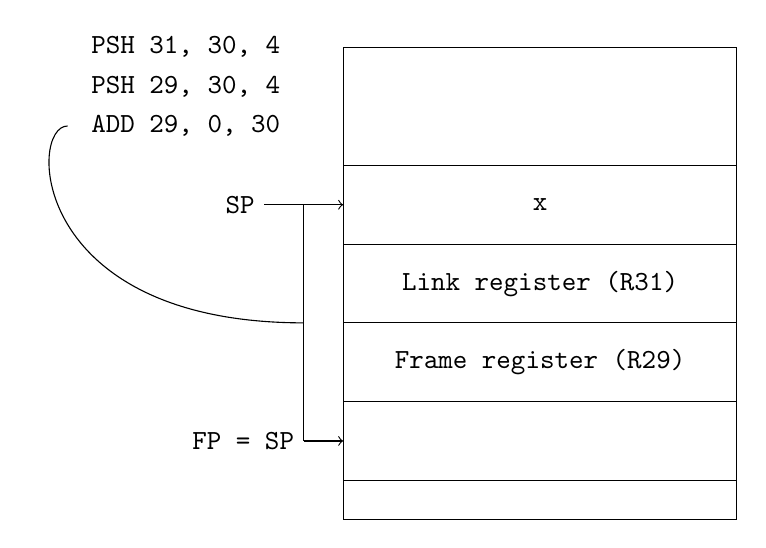
\begin{tikzpicture};
			\draw (4, 0) rectangle (9, 6);

			\draw (4, 0.5) -- (9, 0.5);
			\draw (4, 1.5) -- (9, 1.5);
			\draw (4, 2.5) -- (9, 2.5);
			\draw (4, 3.5) -- (9, 3.5);
			\draw (4, 4.5) -- (9, 4.5);

			\node at (6.5, 4) {\texttt{x}};
			\node at (6.5, 3) {\texttt{Link register (R31)}};
			\node at (6.5, 2) {\texttt{Frame register (R29)}};

			\node at (2, 6) {\texttt{PSH 31, 30, 4}};
			\node at (2, 5.5) {\texttt{PSH 29, 30, 4}};
			\node at (2, 5) {\texttt{ADD 29, 0, 30}};

			\draw[<-] (4, 4) -- (3, 4) node[left] {\texttt{SP}};
			\draw[<-] (4, 1) -- (3.5, 1) node[left] {\texttt{FP = SP}};
			\draw (3.5, 4) -- (3.5, 1);
			\draw (0.5, 5) .. controls (0, 5) and (0, 2.5) .. (3.5, 2.5);
		\end{tikzpicture}
		\caption{Stack snapshot of a function with one argument \texttt{x}.}
		\label{fig:memsnapshotfunc}
	\end{figure}
}
\clearpage

\par{
	\noindent
	\underline{Caller vs. Callee:}
	\par{
		\noindent
		The caller of a function \texttt{f} invokes the function, e.g. \texttt{f(x);}. \newline
		The callee is the function itself, e.g. \texttt{int f(int x) \{ ... \}}. \newline
		The callee can again be a caller if it invokes another function in its body, \newline e.g. \texttt{int f(int x) \{ ... g(x); ... \}}.
	}
}

\par{
	\noindent
	\underline{Declaration vs. Definition:}
	\par{
		\noindent	
		A declaration is inserted into the symbol table of a compiler, e.g. \texttt{int x;}. The declaration tells the compiler that a variable or function exists. \newline
		A definition is the actual value assignment, e.g. \texttt{x = 2;}. A definition can be done multiple times in a source code.
	}
}

\par{
	\noindent
    \underline{Example:}
    \par{
        \noindent
        \begin{tabular}{lll}
            \hline
            C Code              	&   Instructions                &    Additional information                             				\\
            \hline
            \hline
            \rowcolor{blue!25}                
            \texttt{y = x + f(x);}	&   \texttt{LDW 1, 28, -4}     	&   Load \texttt{x}														\\
            \rowcolor{blue!25}
            						&   \texttt{PSH 1, 30, 4}     	&   Save context of \texttt{f}			             					\\
            \rowcolor{blue!25}
									&	\texttt{LDW 1, 28, -4}		&	Load \texttt{x}														\\
            \rowcolor{blue!25}
            						&   \texttt{PSH 1, 30, 4}     	&   Push actual argument(s) for f onto stack		             		\\
            \rowcolor{blue!25}
									&	\texttt{BSR 0, 0, <faddr>}	&	Branch to \texttt{f}												\\
            \rowcolor{blue!25}
            						&   \texttt{\ldots}     		&  	Execute function \texttt{f}						             		\\
            \rowcolor{blue!25}
            						&   \texttt{POP 1, 30, 4}     	&   Restore context of \texttt{f}					             		\\
            \rowcolor{blue!25}
									&	\texttt{ADD 2, 0, 27}		&	Store return value into \texttt{R2}									\\
            \rowcolor{blue!25}
            						&   \texttt{ADD 1, 1, 2}     	&   Actual addition of \texttt{x} and \texttt{f(x)}        				\\
            \rowcolor{blue!25}
									&	\texttt{STW 1, 28, -8}		&	Store result.														\\
			\rowcolor{blue!25}
									&								&	\texttt{-8} because it's the second global variable					\\
            \hline
        \end{tabular}
    }    
}

\subsection*{Heap}

\par{
	\noindent
	Dynamically allocated memory is located on the heap. In C there is the \texttt{malloc}/\texttt{free} combination to accomplish this, in Java there is the \texttt{new} keyword to allocate memory dynamically but no explicit mechanism to deallocate it. Java has a garbage collector which safely deallocates unneeded memory. However, Java provides implicit deallocation mechanisms. The first is to set a reference explicitely to null:
	\begin{verbatim}
        x = new A(); // dynamic allocation
        ...
        ...
        x = null;
        // if no other reference to x exists here
        // x will be deallocated by the garbage collector
	\end{verbatim}
	The second approach uses namespaces. When jumping out from a namespace, every namespace-local variables are unneeded if and only if there are no references from outside. If there are no such references the garbage collector will deallocate these variables:
	\begin{verbatim}
        {
            x = new A();
            ...
            ...
        }
	\end{verbatim}
}

\par{
    \noindent
    The simplest (but most unintelligent) implementation of a dynamic heap allocator is a so-called \textit{bump pointer allocator}. A bump pointer is a pointer which only counts upwards, never downwards. In this case, there is no \texttt{free} to deallocate because it only grows upwards. However, the implementation of \texttt{malloc} is pretty simple and straigh-forward:
    \begin{verbatim}
        void *malloc(int s) {
            LDW 1, 29, 12
            ADD 27, 0, 26
            ADD 26, 26, 1 // R26 = Heap pointer
        }
    \end{verbatim}
    So every time \texttt{malloc} is invoked, these three DLX instructions are executed.
}
